\chapter{Explorarea setului de date}

\section{Descriere}

Acest set de date conţine informaţii despre 284,807 de tranzacţii dintre care 
492 sunt \textbf{frauduloase}. Conţine doar variabile numerice.

Din motive de confidenţialitate, dimensiunea trăsăturilor originale a fost 
redusă folosind \textbf{Principal Component Analysis} (PCA) la 28 de trăsături denumite 
"V1-V28" şi încă 2 trăsături ce nu au fost transformate, anume suma de bani
a tranzacţiei şi timpul relativ, începând de la 0, când aceasta a fost făcută. 
De asemenea, pentru fiecare tranzacţie avem eticheta 0 sau 1, daca este normală 
sau, respectiv, frauduloasă.

\begin{figure}[H]
    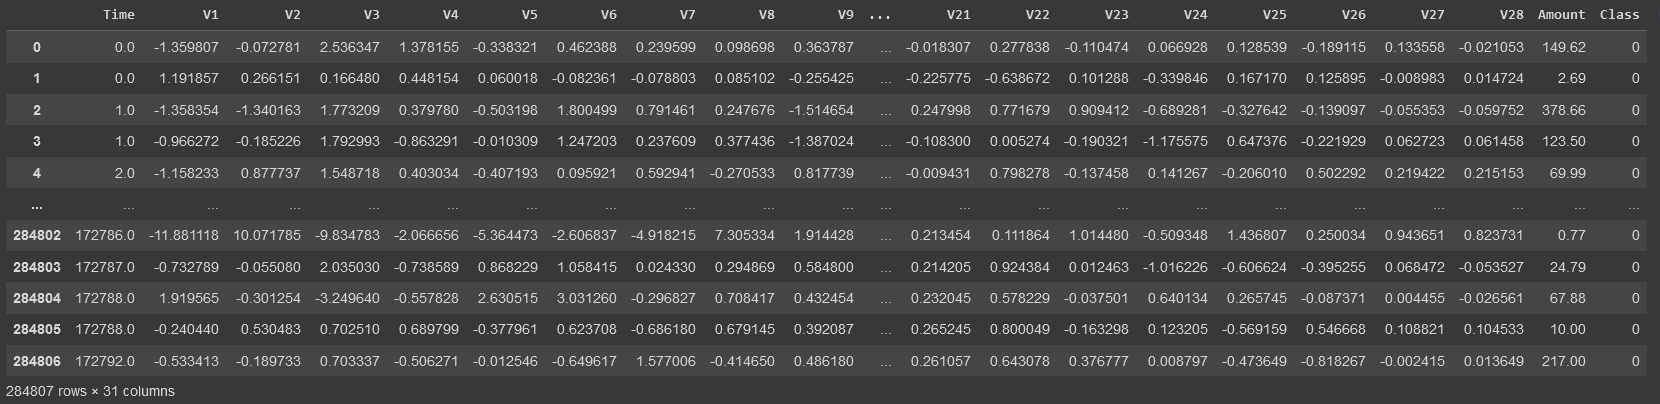
\includegraphics[width=\linewidth]{dataframe.png}
    \caption{Cele 284,807 de tranzacţii}
\end{figure}


\section{Matricea de corelaţie}

\begin{figure}[H]
    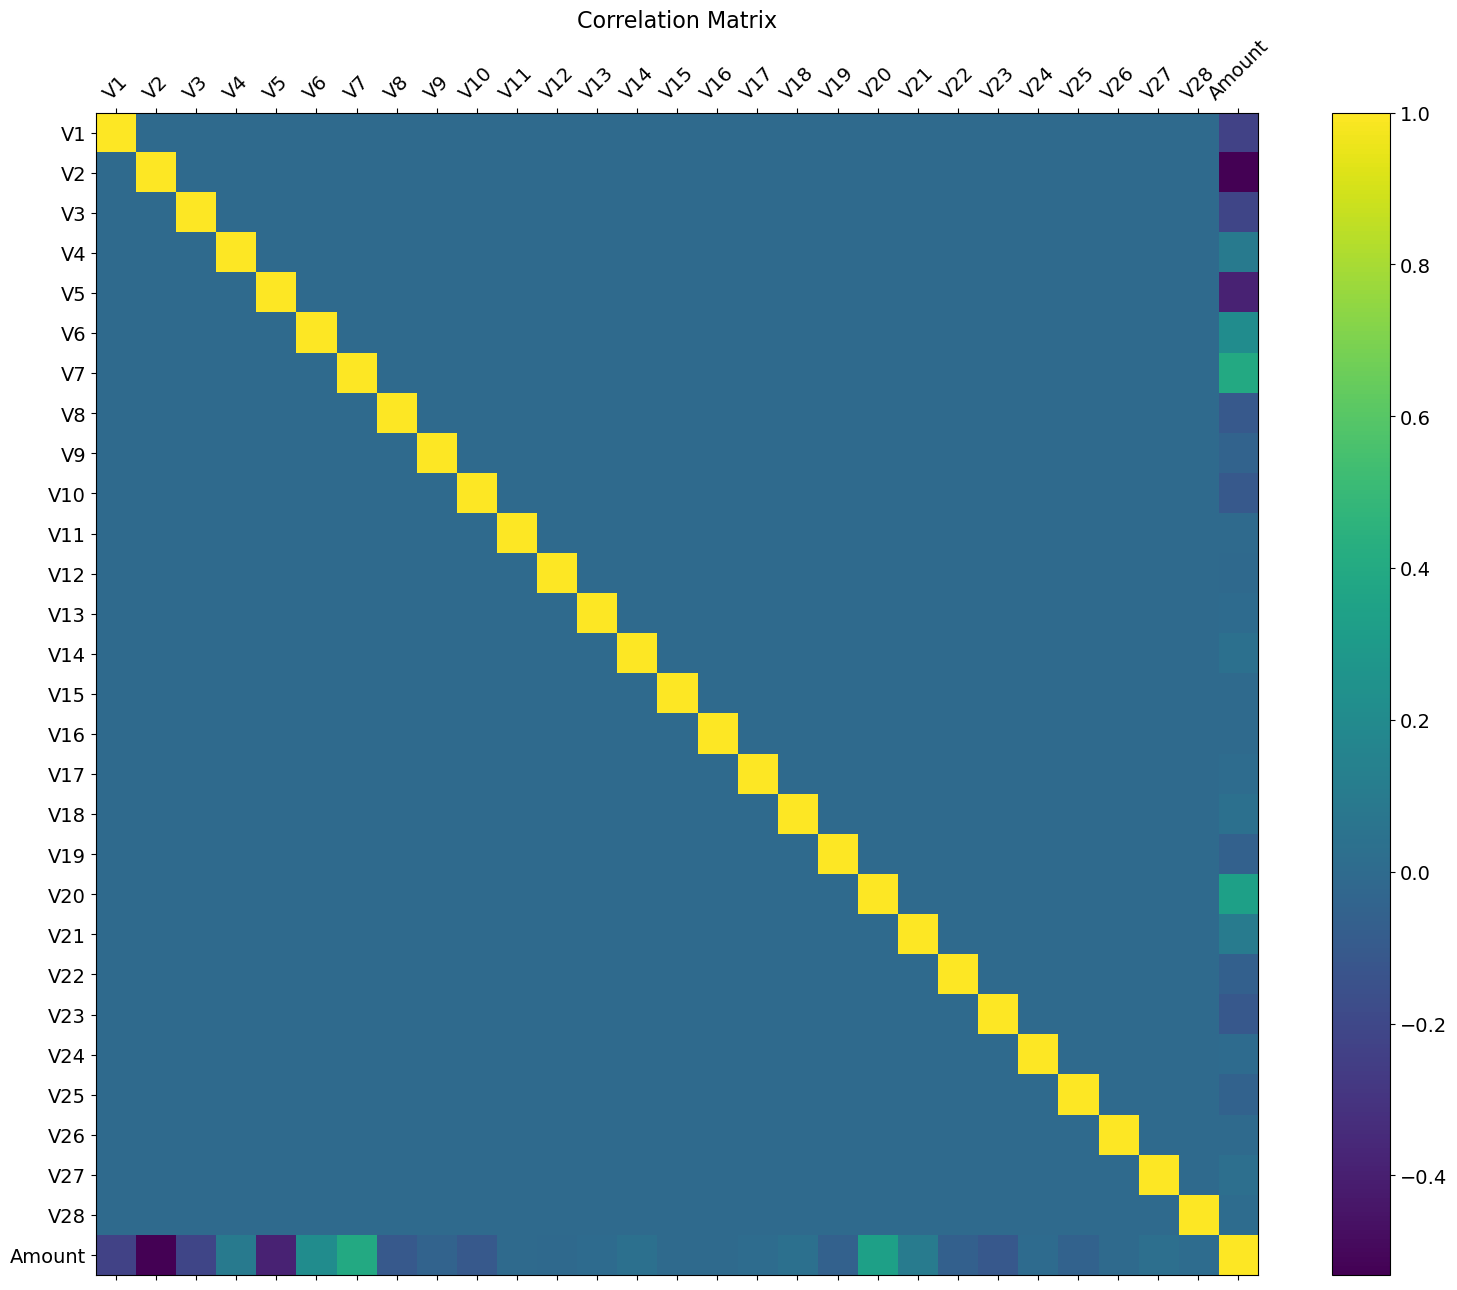
\includegraphics[width=\linewidth]{correlation-matrix.png}
    \caption{Matricea de corelaţie}
\end{figure}

Se observă lipsa corelaţiei între variabilele anonime. Este de aşteptat, totuşi, 
având în vedere că variabilele au fost obţinute prin PCA, care din definiţie generează 
componente \textbf{necorelate liniar}.

Singura corelaţie apare între variabila "Amount" şi restul variabilelor. Corelaţiile
cu o magnitudine semnificativă apar între amount şi V6, V7, V20, cu valoare pozitivă, 
şi între amount şi V1, V2, V5, cu valoare negativă.

\section{Preprocesarea datelor}

\subsection{Eliminăm trăsăturile inutile}

În viaţa reală, data şi ora tranzacţiei ne pot ajuta să depistăm un comportament 
ciudat. Totuşi, aceste informaţii sunt relevante numai atunci când am monitorizat
pe o perioada de măcar câteva zile activitatea din contul/cardul respectiv pentru a 
stabili ce reprezintă un comportament "normal".

În cazul nostru, nu avem la dispoziţie nici măcar data şi ora exactă. Prin urmare, vom
elimina timpul din fiecare observaţie.

De asemenea, eliminăm etichetele. Acestea sunt utile numai la testare pentru a analiza 
performanţa şi la alegerea setului de antrenare. Metodele utilizate în această lucrare
sunt exclusiv \textbf{nesupervizate}, deci nu avem nevoie de etichete la procesul de antrenare.

\subsection{Validarea încrucişată}

Împărţim setul de date, salvând $75\%$ pentru antrenare. Din \textbf{setul de antrenare}, 
extragem toate
datele cu eticheta de anomalie şi le mutăm în porţiunea de $25\%$ rămasă de la pasul anterior.
Apoi, ultima porţiune este împărţită la rândul ei în jumătăţi egale ce vor servi ca set de validare, respectiv testare.

Facem acest lucru deoarece algoritmii prezentaţi "învaţă" structura datelor normale şi, ideal,
nu am vrea niciun fel de anomalie în setul de antrenare. În practică, este o şansă destul de 
mare ca setul de antrenare să fie \textbf{"contaminat"} cu un procent mic de anomalii, fiind dificil 
să garantăm \textbf{"puritatea"} datelor. Totuşi, am decis să presupunem că nu există nicio eroare 
în datele noastre pentru a păstra un număr mai mare de anomalii în setul de validare şi cel de 
testare, pe care să evaluăm performanţa modelelor.

De asemenea, o tehnică des utilizată în împarţirea setului de date pentru metode supervizate 
este \textbf{stratificarea} ce ne conferă o proporţie a claselor, aproximativ egală cu 
cea din setul iniţial, în porţiunile
de antrenare, validare şi testare. Acest lucru este important pentru a ne asigura că fiecare 
clasă este reprezentată corespunzător în eşantionul nostru. În cazul detecţiei anomaliilor, 
o vom ignora deoarece avem doar o singură clasă de referinţă, anume cea normală, la antrenare. 
Datele etichetate ca fiind anomalii sunt utile doar la testare.

\textbf{Setul de validare} va fi folosit pentru alegerea hiperparametrilor optimi, în timp ce 
\textbf{setul de testare} va fi folosit la final pentru a face o comparaţie imparţială 
a performanţei modelelor.

\subsection{Scalare}

Având în vedere că nu cunoaştem dimensiunile, unităţile de măsură şi nici 
numele variabilelor aleatoare asociate punctelor, este indicat să scalăm 
datele. Uneori poate fi util să lăsăm punctele aşa cum sunt, dar aceasta ar necesita 
o decizie informată pe baza importanţei variabilelor în calcularea 
distanţei între puncte sau pe baza 
relevanţei unităţilor variabilelor, de exemplu. 

În lipsa acestori factori, vom standardiza datele, adică  
\textbf{vom scădea media şi vom împărţi la deviaţia standard}, operaţie aplicată 
fiecărui punct. Aceasta are rolul de a centra variabilele şi de a obţine varianţă
unitară pe fiecare variabilă în parte. 
Media şi deviaţia standard sunt obţinute din setul de antrenare. Le folosim pe acestea 
să transformăm setul de validare, cât şi pe cel de testare. Astfel, fiecare trăsătură 
$x_{i}$ va fi inlocuită de o noua trăsătură $x_{i}'$:

$$x_{i}' = \frac{x_{i} - \mu_{i}}{\sigma_{i}}$$
unde $\mu_{i}$ este media: 

$$\mu_{i} = \frac{1}{m} \sum_{j=1}^{m} x_{i}^{(j)}$$
şi $\sigma_{i}$ este deviaţia standard: 

$$\sigma_{i} = \sqrt{ \frac{1}{m} \sum_{j=1}^{m} (x_{i}^{(j)} - \mu_{i}) ^ 2 }$$ 
calculate luând trăsăturile $x_{i}$ din toate cele $m$ observaţii din setul de antrenare.

\begin{figure}[H]
    \centering
    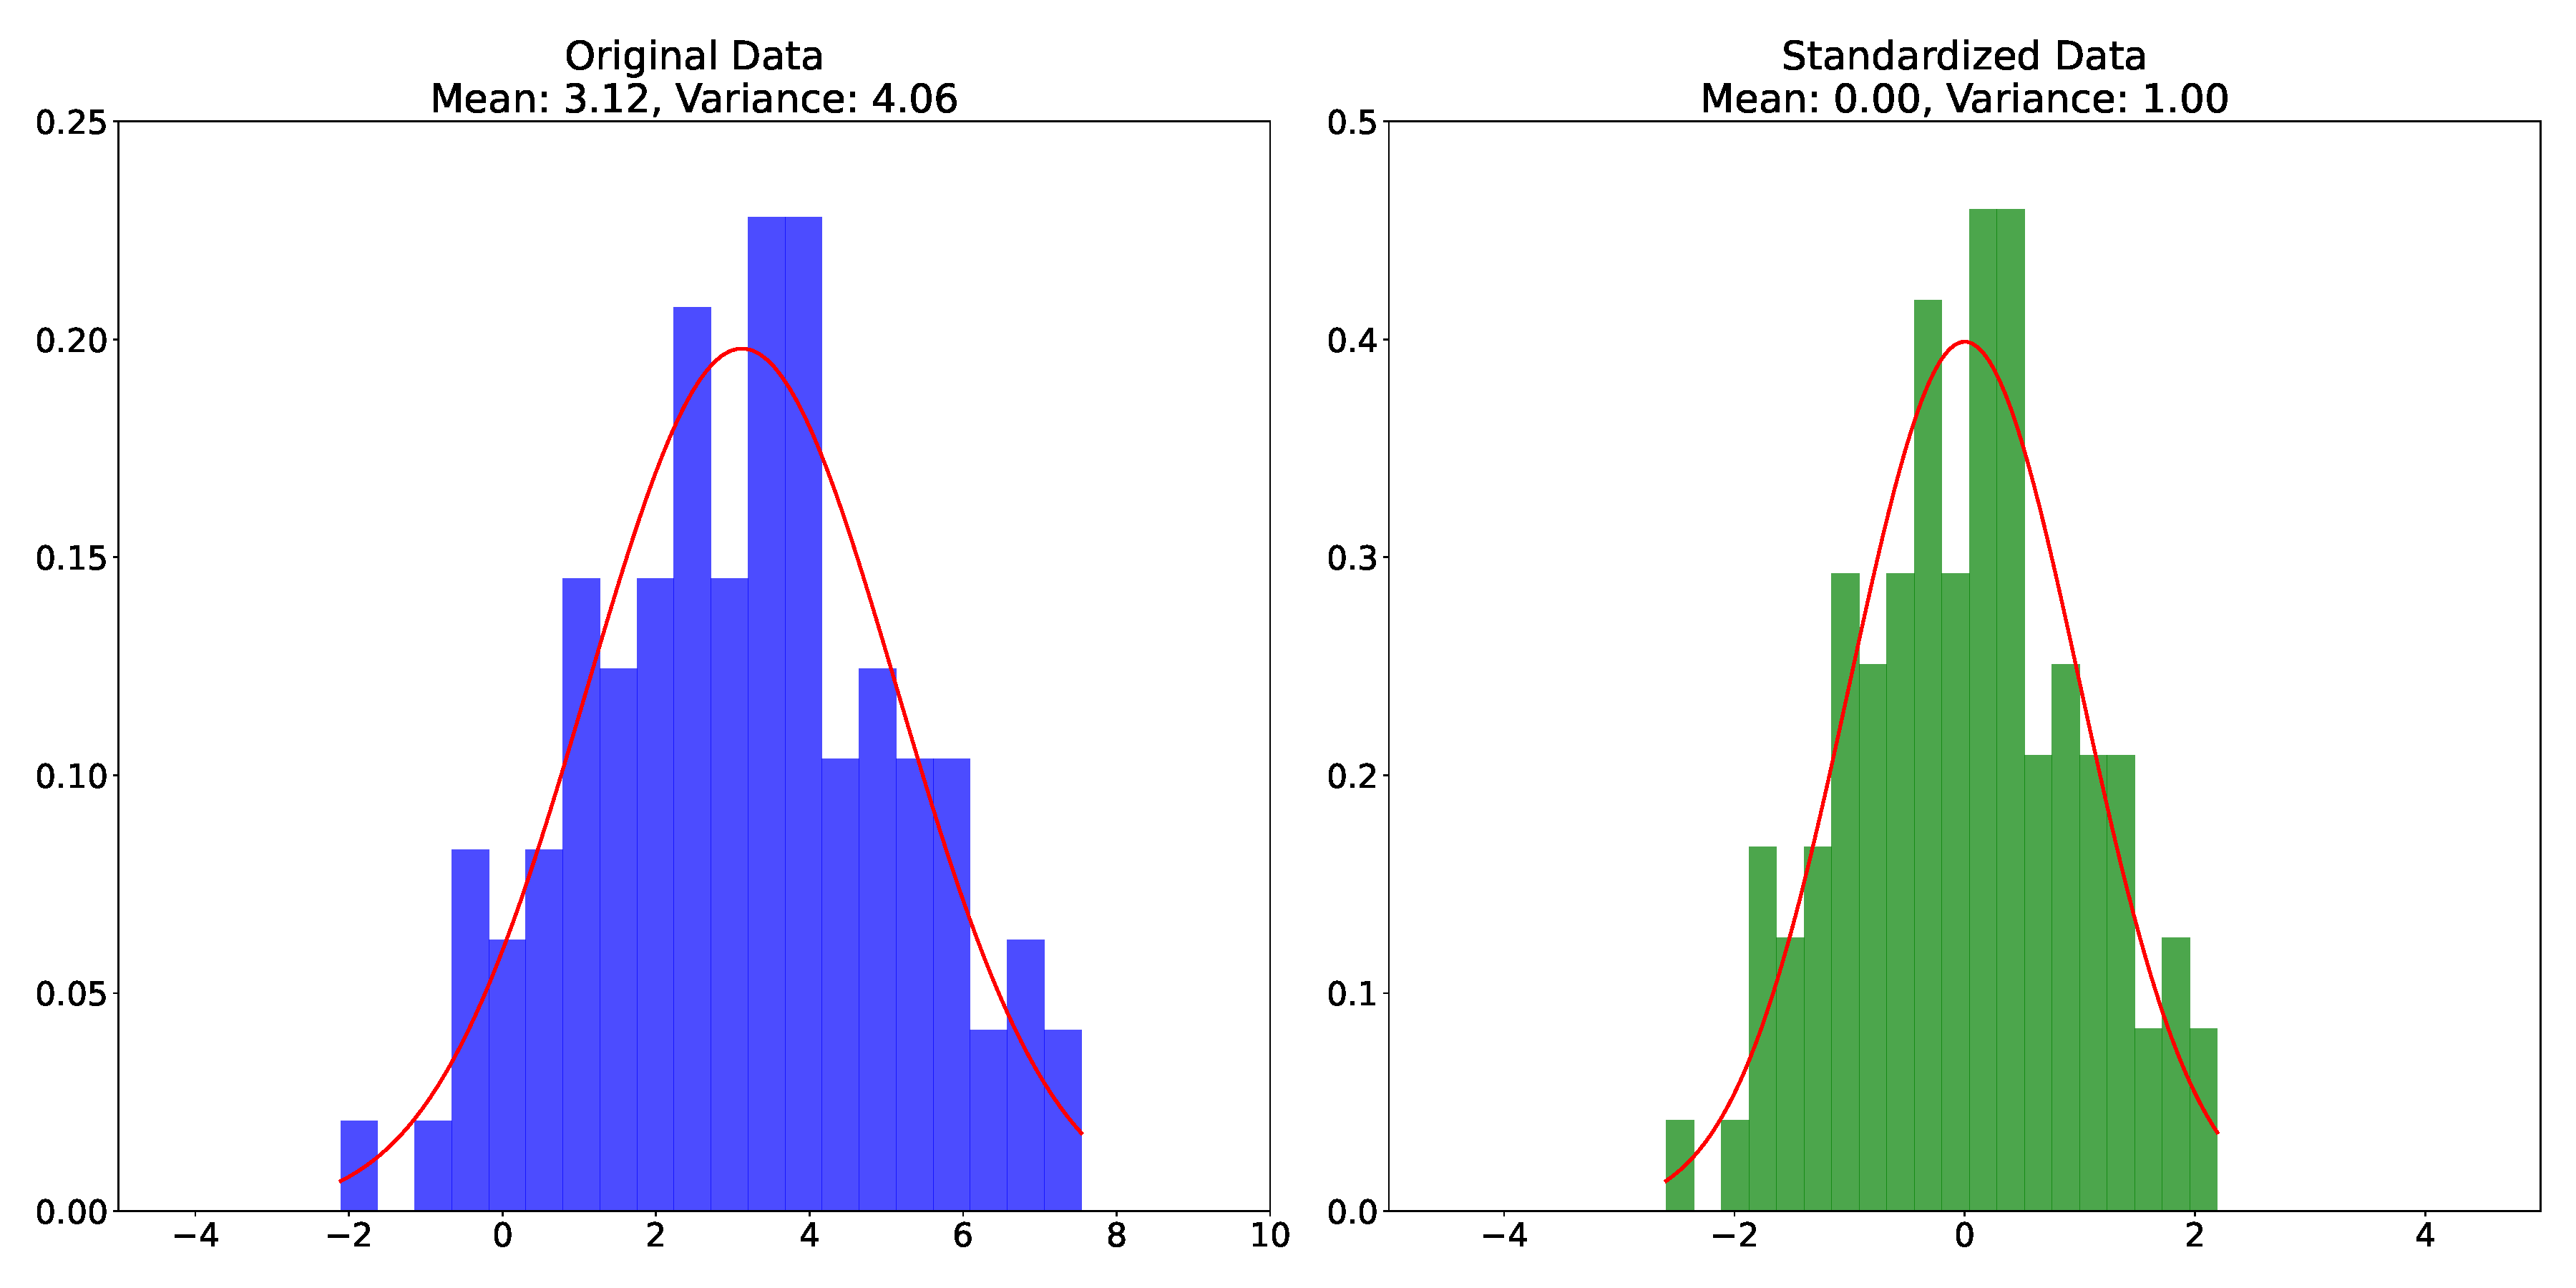
\includegraphics[width=\linewidth]{images/standardiaztion.pdf}
    \caption{Media devine 0, varianţa devine 1}
\end{figure}